
\documentclass[11pt,a4paper]{article}

\usepackage[utf8]{inputenc} 
\usepackage[T1]{fontenc} 
\usepackage{lmodern}
\usepackage{tcolorbox}
\usepackage[german]{babel}

\usepackage{fourier}
\setlength{\parindent}{0pt}
\setlength{\parskip}{1ex plus 0.5ex minus 0.5ex}

\usepackage{amsmath} 


\usepackage{graphicx} 

\usepackage[section]{placeins}
\usepackage{booktabs}


\usepackage{hyperref}
\hypersetup{
	colorlinks,
	citecolor=red,
	filecolor=black,
	linkcolor=black,
	urlcolor=black}
\graphicspath{}

\begin{document}
	

{
	\centering 
	\large 
	Physiklabor für Anfänger*innen \\
	Ferienpraktikum im Sommersemester 2018 \\[4mm]
	\textbf{\LARGE 
		Versuch 14: Streuversuch
	} \\[3mm]
	(durchgeführt am 05.10.2018 bei Assistentin Julia Müller) \\
	Ye Joon Kim, Marouan Zouari\\
	\today \\[10mm]
}

\tableofcontents
\newpage
\section{Einleitung}
Mit einem elastischen Stoß spricht man von einer Kollision, wobei die Summe der kinetischen Energien beide Objekt erhalten ist. Für einen nicht-zentraler Stoß zwischen zwei kugeln werden beide Kugeln in bestimmten Richtungen gestreut. Für diesen Experiment werden Stöße zwischen einem Kugel und einem statischen Zylinder untersucht. Mit Geometrie kann  der folgende Zusammenhang leicht hergeleitet werden (Siehe Abbildung 1, Teil 2). Dieser Zusammenhang koppelt der Winkel $\beta$ zu dem Stoßparameter $b$, der Abstand von dem Flugbahn der Kugel zum dazu parallelen Durchmesser des Streuapparats. 

$$\sin\beta = \frac{b}{r+R}$$
wobei $\beta$ der Einfalls- und Ausfallswinkel relativ zum Flächennormale der Kollisionspunkt, $R$ der Radius des Zylinders und $r$ der Radius der Kugels sind. 

Der Streuwinkel kann mit der Annäherung $\widearc{DB}\approx b$ so geschrieben werden:
$$\theta = \frac{\widearc{AB}-b}{s}$$
Und da $\theta + 2\beta = \pi$, kann $\theta$ in Terme von $b$, $r$ und $R$ ausgedruckt werden. 
$$\sin{\frac{\pi-\theta}{2}}=\cos{\frac{\theta}{2}}=\frac{b}{r+R}$$

Das Ziel des Versuchs ist deshalb es, der Radius des Zylinders durch die Messungen der Streuwinkel zu bestimmen. 


\begin{figure}
	\centering
	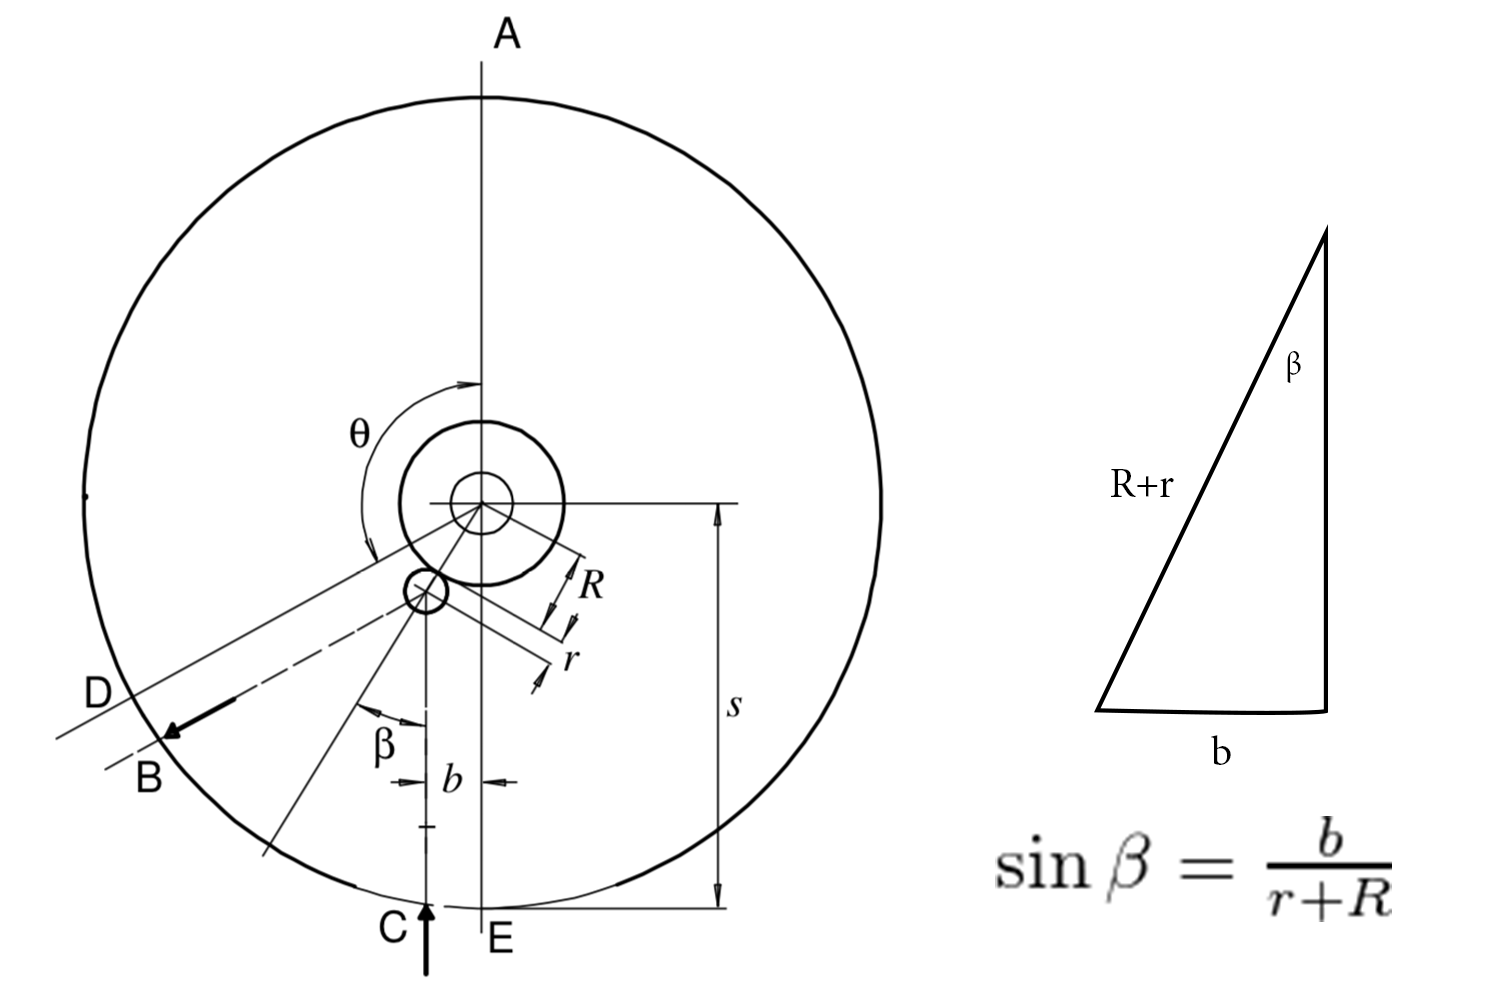
\includegraphics[width=\linewidth]{Abb1}
	\caption{Geometrie der Streuungen (,,Versuchsanleitungen'').}
\end{figure}

\section{Aufbau}
\begin{figure}
	\centering
	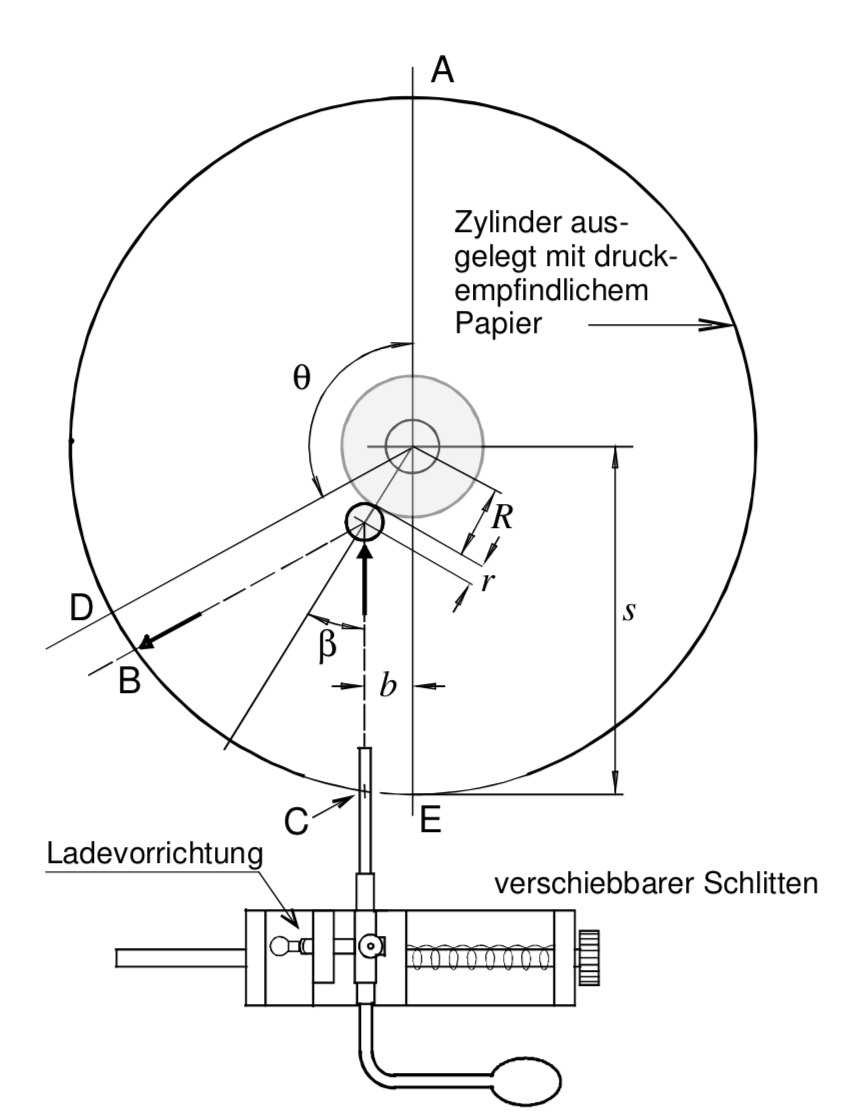
\includegraphics[scale=0.4]{Abb3}
	\caption{Versuchsaufbau (,,Versuchsanleitungen''.)}
\end{figure}

Der Aufbau dieses Versuchs besteht aus einem großen Hohlzylinder mit einem kleineren Hohlzylinder in der Mitte. Auf einer Seite des großen Zylinders gibt es eine Öffnung, wodurch die kleine Kugeln mit einem verschiebbaren Luftdruckkugelbeschleunigungsgerät geschossen werden können. Die innere Seite des Zylinders wurde mit druckempfindlichem Papier gelegt (Siehe Abbildung 2). Es wurden auch einen Lineal und Maßband verwendet. 

\section{Durchführung}
Zuerst wurde der Durchmesser des Innenraums des großen Hohlzylinders mit einem Maßband gemessen. Die Position $\theta = 0$ wurde auch mit dem Maßband bestimmt und auf das Papier markiert. Das Kugelschießgerät wurde dann so verschoben, sodass die geschossenen Kugel zurückreflektiert werden. Die Position des Geräts wurde dann als $b_0$ aufgenommen. Das Gerät wurde danach nach rechts verschoben, ihre Position aufgenommen und mit 20 Kugeln geladen. Die Kugel wurden dann mithilfe des Ballonförmigen Bauteils geschossen. Die Markierungen auf dem Paper wurde dann gekennzeichnet. Dieser Prozess wurde für acht andere Positionen des Geräts auf beide Seiten des Targetzylinders wiederholt. Das druckempfindliche Papier wurde dann entnommen und die mittleren Positionen der Markierungen sowie deren Streuung abgeschätzt und auf dem Papier gezeichnet. 


\section{Auswertung und Fehleranalyse}

Die Werte für $b$ und der Mittelwerte von $\widearc{AB}$ sowie deren Unsicherheiten sind in Tabelle 1 zu sehen:
\\\
\begin{table}[h]
	\centering
	\begin{tabular*}{0.50\textwidth}{@{\extracolsep{\fill}}ccccc}
		\toprule
		$b$ & $\Delta b$ & $\overline{\widearc{AB}}$ & $s_{\widearc{AB}}$ & $u_{\overline{\widearc{AB}}}$ \\
		cm & cm & cm &cm& cm\\
		\midrule
		-0,5 & 0,1 & -89,3 & 0,4 & 0,2\\
		-0,8 & 0,1 & -84,7 &0,6& 0,2\\
		-1,2 & 0,1 & -76,6 &0,6& 0,2\\
		1,2 & 0,1& 78,9 &0,9& 0,2 \\
		1,7 & 0,1 & 67,0 &1,3& 0,3 \\
		2,2 & 0,1 & 53,2 &1,2& 0,3 \\
		-1,8 & 0,1 & -59,7 &1,3& 0,3 \\
		2,7 & 0,1 & 37,9 &1,4& 0,3\\
		\bottomrule
\end{tabular*}
\caption{Die gemessenen Werte für $b$, $\overline{\widearc{AB}}$ und deren Unsicherheiten}
\end{table}

\begin{tcolorbox}[colback=white]
\subsection{Rechenweg}
Für die Unsicherheit von $b$ wurde die vereinfachte gaußsche Fehlerfortpflanzung benutzt. Da $b$ sich um eine Differenz handelt, ist:
$$\Delta b = \sqrt{(\Delta b_n)^2 + (\Delta b_0)^2}$$

Für die Unsicherheiten von $\overline{\widearc{AB}}$ wurde die abgeschätzten Standardabweichungen durch einen Faktor $\sqrt{n}$ geteilt, da es geht um einen Mittelwert. Es wurden auch die Ablesefehler von $\widearc{AB}$ und von dem Punkt $A$ berücksichtigt. Deswegen beträgt der gesamte Fehler von $\overline{\widearc{AB}}$:
$$
u_{\overline{\widearc{AB}}} = \sqrt{\left(\frac{s_{\widearc{AB}}}{\sqrt{n}}\right)^2+u_\textrm{Ab}^2+u_A^2}
$$
In diesem Fall waren $u_\textrm{Ab}$ und $u_A$ beide 0,1 cm.
\end{tcolorbox}


Danach wurde die $\overline{\widearc{AB}}$ Werte in $\theta$ umgewandelt.
\\\
(Siehe Tabelle 2).

\newpage
\begin{table}[h]
	\centering
	\begin{tabular*}{0.50\textwidth}{@{\extracolsep{\fill}}cccc}
		\toprule
		$|b|$ & $\Delta b$ & $|\theta|$ & $u_\theta$  \\
		cm & cm & rad & rad \\
		\midrule
		0,5 & 0,1 & 2,812 & 0,010\\
		0,8 & 0,1  &2,668& 0,009\\
		1,2 & 0,1  &2,413& 0,009\\
		1,2 & 0,1 &2,447& 0,010\\
		1,7 & 0,1  &2,057& 0,012\\
		2,2 & 0,1  &1,606& 0,011\\
		1,8 & 0,1  &1,824& 0,011\\
		2,7 & 0,1  &1,187& 0,011\\
		\bottomrule
	\end{tabular*}
\caption{Die Werte für $\theta$ und ihre Unsicherheiten}
\end{table}

\begin{tcolorbox}[colback=white]
\subsection{Rechenweg}
Da $\theta = \frac{\widearc{AB}-b}{s}$, wurde die gaußsche Fehlerfortpflanzung verwendet.
Sei:
$$\theta(\widearc{AB},s,b) = \frac{\widearc{AB}-b}{s}$$
Dann sind:
$$\frac{\partial \theta}{\partial \widearc{AB}} = \frac{1}{s}$$
$$\frac{\partial \theta}{\partial s} = \frac{-\widearc{AB}+b}{s^2}$$
$$\frac{\partial \theta}{\partial b} = -\frac{1}{s}$$
 deswegen ist
$$u_\theta = \sqrt{(\frac{\partial \theta}{\partial \widearc{AB}}u_{\widearc{AB}})^2+(\frac{\partial \theta}{\partial s}\Delta s)^2+(\frac{\partial \theta}{\partial b}\Delta b)^2}$$
\end{tcolorbox}

Die Werte für $\cos{\frac{\theta}{2}}$ wurden dann gegen $\left|b\right|$ aufgetragen (Siehe Abbildung 3). 
\begin{figure}[h]
	\centering
	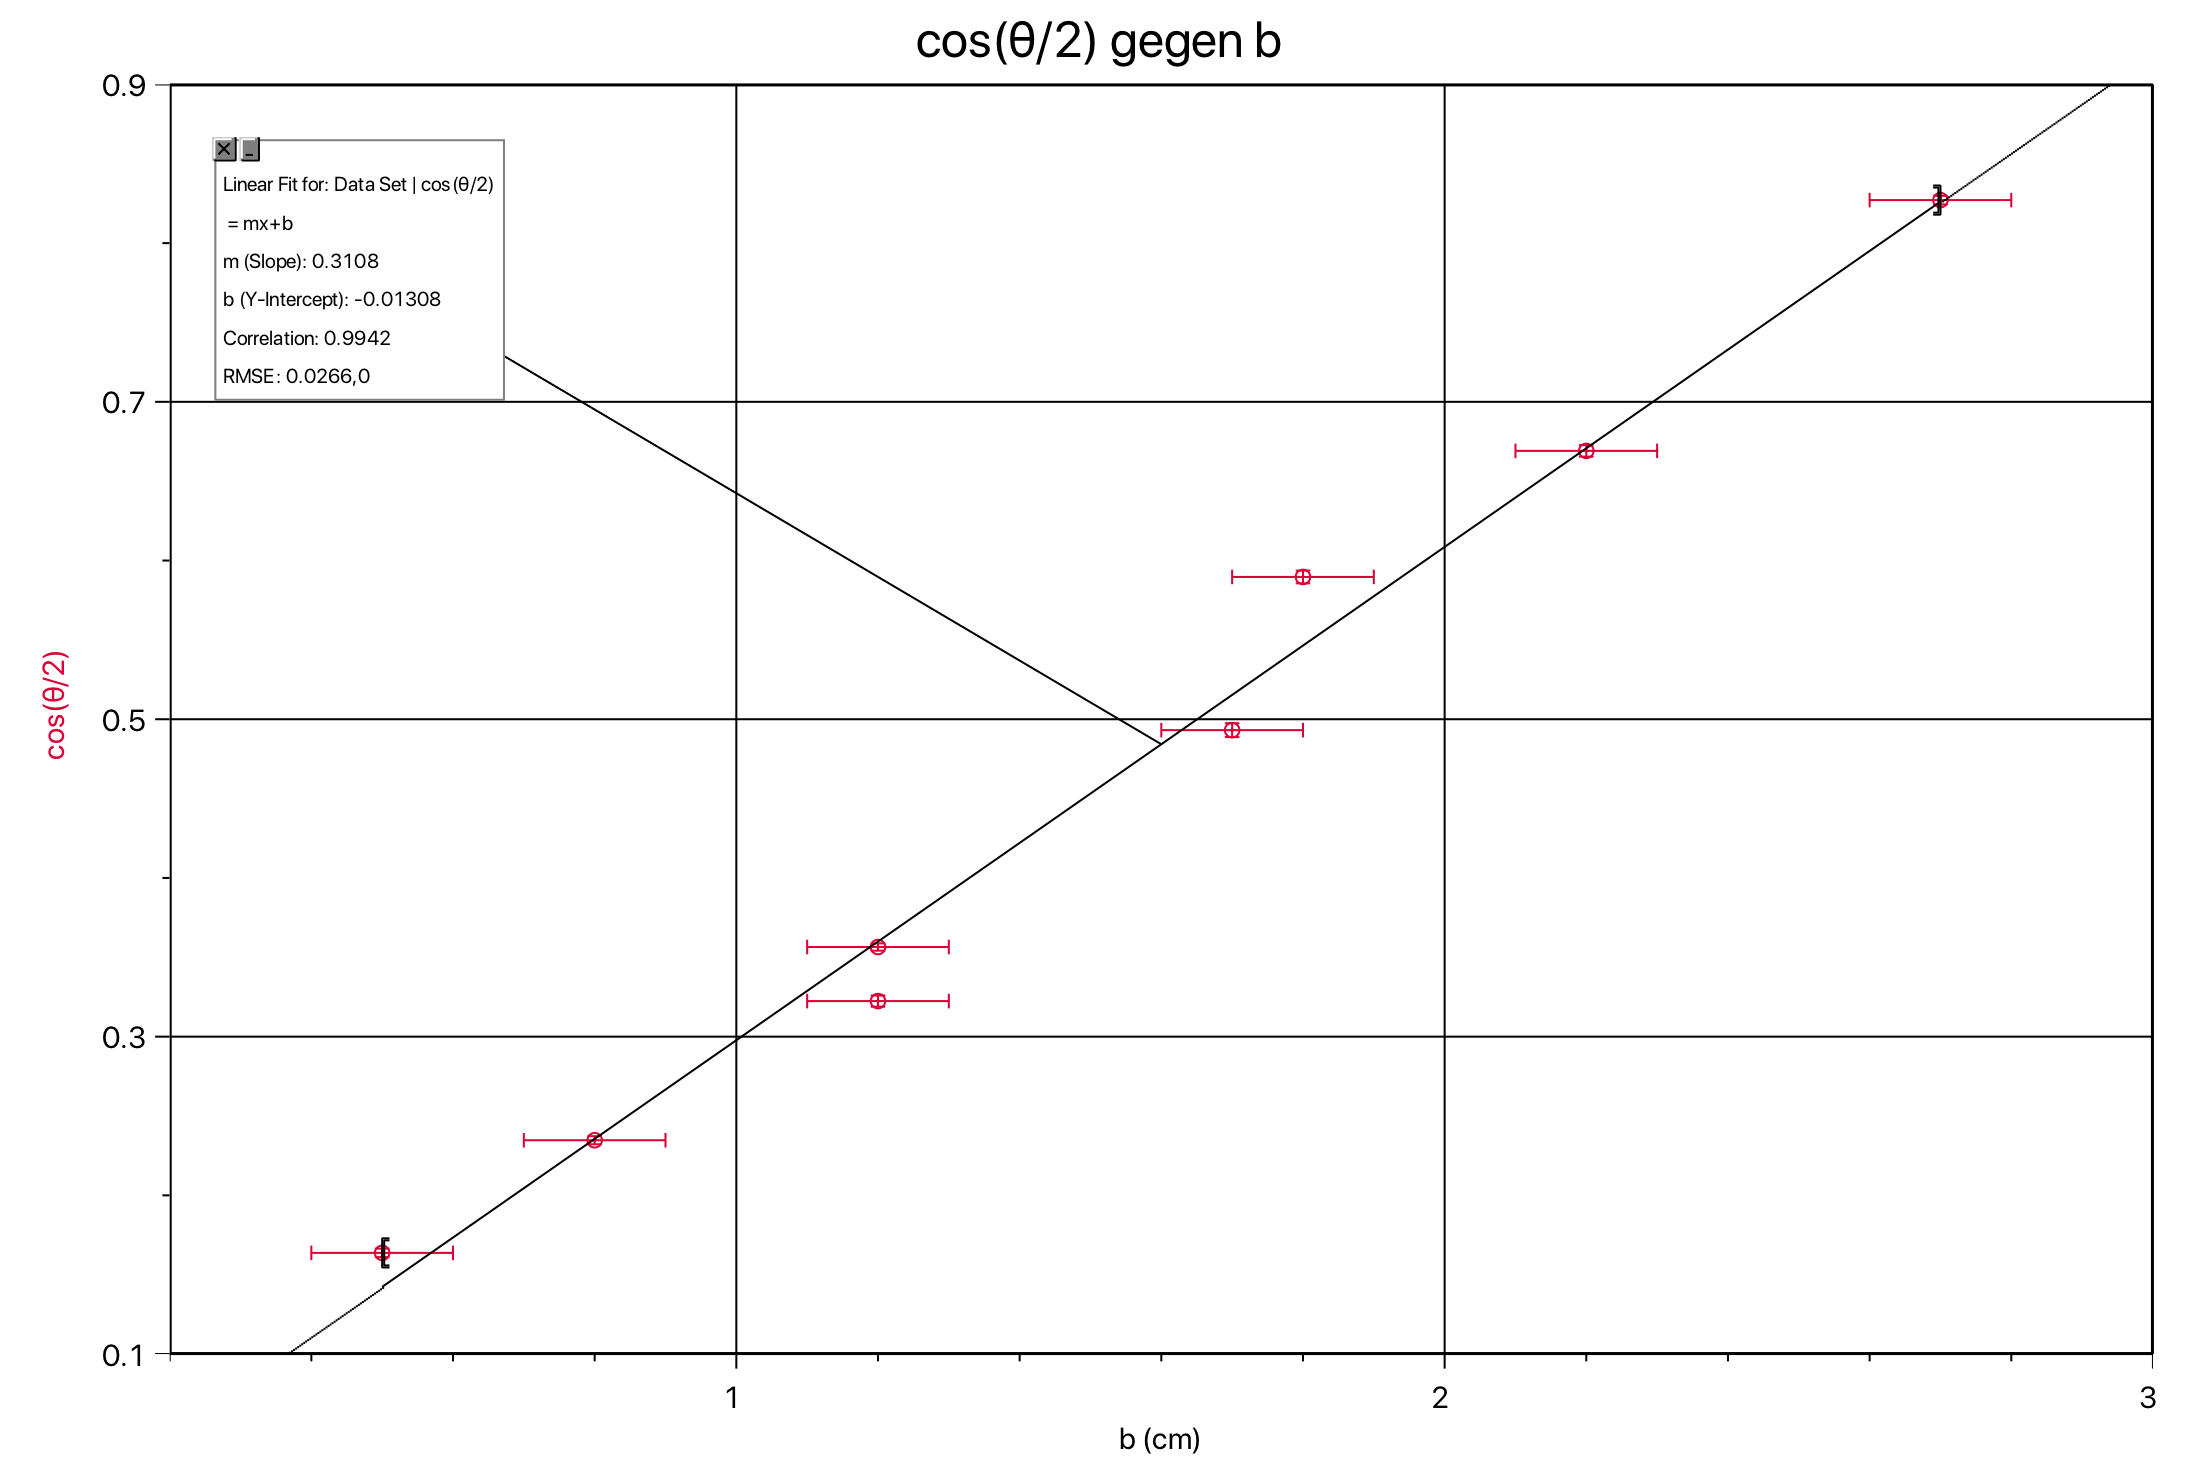
\includegraphics[width=\linewidth]{Abb2}
	\caption{Eine Auftragung von $\cos{\frac{\theta}{2}}$ gegen $|b|$ (y Fehlerbalken wegen kleiner Größe nicht abgebildet}
\end{figure}

Da $\cos{\frac{\theta}{2}}$ linear zu $b$ ist, kann der Zusammenhang dazwischen in so einer Form:
$$ \cos{\frac{\theta}{2}} = a+m\cdot b$$
geschrieben werden. $m$ entspricht deshalb dem Wert $\frac{1}{r+R}$. Die Werte und Unsicherheiten für $a$ und $b$ wurden mit einem Excel-Dokument berechnet:
$$ a = (-0,01 \pm 0,02) $$
$$ m = (0,318 \pm 0,012) \textrm{cm}^{-1} $$

\begin{tcolorbox}[colback=white]
\subsection{Rechenweg}
Obwohl in der Abbildung unsichtbar, wurden die Unsicherheiten der $\cos{\frac{\theta}{2}}$ mit der gauß'schen Fehlerfortpflanzung berechnet. 
Mit:
$$f(\theta) = \cos\frac{\theta}{2}$$
ist
$$\frac{\partial f}{\partial \theta} = -\frac{1}{2}\sin\frac{\theta}{2}$$
Deshalb ist die Unsicherheit:
$$u_{\cos\frac{\theta}{2}} = \frac{\partial f}{\partial \theta}\cdot u_\theta$$

Für die Bestimmung der Werte und Unsicherheiten für $a$ und $m$ wurden die folgenden Formel benutzt:
$$a = \frac{
	\sum x_i^2 \sum y_i - \sum x_i \sum x_iy_i
}{
	n \sum x_i^2 - (\sum x_i)^2
}$$
$$ m = \frac{
	n\sum x_iy_i-\sum x_i \sum y_i
}{
	n \sum x_i^2 - (\sum x_i)^2
}$$
\end{tcolorbox}
\begin{tcolorbox}[colback=white]
$$u_a = s\cdot \sqrt{
	\frac{
		\sum x_i^2
	}{
		n\sum x_i^2 - (\sum x_i)^2
}}$$

$$u_m = s\cdot \sqrt{
	\frac{
		n
	}{
		n\sum x_i^2 - (\sum x_i)^2
}}$$
Mit $x = b$, $y = \cos\frac{\theta}{2}$ und $s = \sqrt{
	\frac{1}{n-2}\sum [y_i-(a+mx_i)]^2}$
	
\end{tcolorbox}

Jetzt kann der Wert für $s$ mit der Steigung $m$ berechnet werden:
$$ s = (2,92 \pm 0,12) \textrm{cm} $$
Die Durchmesser ist deshalb:
$$ d = (5,8 \pm 0,2) \textrm{cm}$$
\begin{tcolorbox}[colback=white]
\subsection{Rechenweg}
Für die Berechnung der Wert von  $R$ :
$$ m= \frac{1}{R+r}$$
$$ => R = \frac{1}{m}-r$$ 


Für die Berechnung der Unsicherheit wurde die Gaußsche Fehlerfortpflanzung benutzt. Mit
$$R(m) = \frac{1}{m}-r$$ 
ist
$$\frac{\partial R}{\partial m} = -\frac{1}{m^2}$$
Die Unsicherheit von $R$ ist deshalb:
$$u_R = \left|\frac{\partial R}{\partial m}\cdot u_m\right|$$

	
\end{tcolorbox}
\section{Diskussion}


\subsection{Diskussion "uber die gefundene Werten}
Der direkt gemessene Durchmesser des Zylinders lautet :
$$(5,8\pm0,1) \textrm{cm}$$

und der durch dieses Experiment bestimmte Wert ist: 
$$(5,8\pm0,2) \textrm{cm} $$

Ohne ihr $t$-Wert bestimmen zu müssen, kann es sofort gesehen werden, dass die Beide Werte miteinander übereinstimmen. Die Relative Unsicherheit des Wertes beträgt ungefähr 2\%, was relativ klein ist. Deshalb ist dieses Ergebnis auch aussagekräftig und kann als Beweis für den in der Einleitung erwähnten Zusammenhang dienen. 
 
\subsection{Systematische und statistische Fehler}
Der verwendete Aufbau war auf dem horizontalen Tisch nicht ganz stabil und konnte hin und her wackeln, falls eine Seite nicht mit einem kleinen Objekt unterstützt wurde. Diese Instabilität ist eine Quelle für statistische Fehlern, da das ganze Experiment und die Berechnung annehmen, dass das gesamte System horizontal liegt. 

Ein Weiterer statistischer Fehler war es, dass der Luftdruck des Schießgeräts nicht immer konstant war, da er von Hand erzeugt werden musste. Das kann beeinflussen, wo das Projektil auf das Papier auftrifft. 

Weil der Stoßparameter $b$ einen relativ kleinen Wert hat, wurde die Strecke $\widearc{DB}$ bei der Herleitung der Formeln zu $b$ angenähert (Siehe Abbildung 1). Das bedeutet, dieser Kreisbogen wurde als eine gerade Linie statt einer Kurve betrachtet. Daher für größere $b$ Werte sind die berechneten $\theta$ Werte kleiner als die tatsächlichen Werte, und das führt zu einem systematischen Fehler. 

\section{Literatur und Bildquellen}
,,Versuchsanleitung zum Physiklabor für Anfänger*innen.'' Albert-Ludwigs-Universität Freiburg. 
\section{Anhang}
Siehe Scans
\end{document}
